\afterpage{\blankpage}
\newpage
\afterpage{\blankpage}
\newpage
\chapter{Presentaci\'on y an\'alisis de resultados}
\section{Distancias de profundidades recomendadas entre el atleta y el sensor} \label{res:idMov}
En la siguiente tabla se muestra un resumen general de las caracter\'isticas de la muestra de cada equipo deportivo, en ella se describe la altura promedio y las distancias recomendadas para ejecutar correctamente el seguimiento del esqueleto (renderizaci\'on completa del esqueleto humano), dichos datos fueron capturados por el sensor Kinect a una altura de 0.70 metros desde el suelo y tomando como punto de referencia, la cadera central de cada atleta:
\begin{table}[H]
\begin{center}
\caption{Distancias de profundidades recomendadas para el funcionamiento del seguimiento del  esqueleto}
\label{tab:depthCalculation}
\begin{tabular}{lllll}
\hline
\multicolumn{3}{|c|}{Caracter\'isticas generales} & \multicolumn{2}{l|}{\begin{tabular}[c]{@{}l@{}}Distancias de profundidades recomendadas \\ entre el usuario y el sensor\end{tabular}} \\ \hline
\multicolumn{1}{|l|}{Deporte} & \multicolumn{1}{l|}{\begin{tabular}[c]{@{}l@{}}Altura promedio\\ (metros)\end{tabular}} & \multicolumn{1}{l|}{\begin{tabular}[c]{@{}l@{}}Desviaci\'on est\'andar\\ de la altura (metros)\end{tabular}} & \multicolumn{1}{l|}{\begin{tabular}[c]{@{}l@{}}M\'inima\\ (metros)\end{tabular}} & \multicolumn{1}{l|}{\begin{tabular}[c]{@{}l@{}}M\'axima\\ (metros)\end{tabular}} \\ \hline
\multicolumn{1}{|l|}{Tenis de mesa} & \multicolumn{1}{l|}{1.302435} & \multicolumn{1}{l|}{+/- 0.088683} & \multicolumn{1}{l|}{3.505103} & \multicolumn{1}{l|}{3.990376} \\ \hline
\multicolumn{1}{|l|}{Animaci\'on} & \multicolumn{1}{l|}{1.342471} & \multicolumn{1}{l|}{+/-0.059301} & \multicolumn{1}{l|}{2.763813} & \multicolumn{1}{l|}{3.411942} \\ \hline
\multicolumn{1}{|l|}{Taekwondo} & \multicolumn{1}{l|}{1.373372} & \multicolumn{1}{l|}{+/-0.098490} & \multicolumn{1}{l|}{2.556640} & \multicolumn{1}{l|}{3.869427} \\ \hline
\multicolumn{5}{l}{\textbf{Fuente:} Datos capturados por los atletas}
\end{tabular}
\end{center}
\end{table}
\section{Muestras de fotogramas del movimiento} \label{res:fotogramas}
En esta secci\'on se realiz\'o por cada equipo deportivo, una tabla en donde se muestra las  fotogramas del seguimiento del  esqueleto de cada atleta (utilizados para los entrenamientos y los testeos del algoritmo Random Forest Regression), con la finalidad de mostrar distintas formas correctas para ejecutar un paso (de acuerdo al profesional). As\'i mismo por cada fotograf\'ia se muestra cuatros elementos importantes:
\begin{itemize}
\item El fondo de color negro.
\item El piso representado por cuadros de colores grises.
\item La figura del atleta figurado por una sombra de color gris.
\item El seguimiento del esqueleto conformado por puntos (articulaciones) y l\'ineas de color blanco (uni\'on de dos articulaciones).
\end{itemize}
\begin{figure}[H]
	\caption{Fotogramas de 6 sujetos del equipo de tenis de mesa}
	\label{fig:fotogramaTenis}
	\centering
	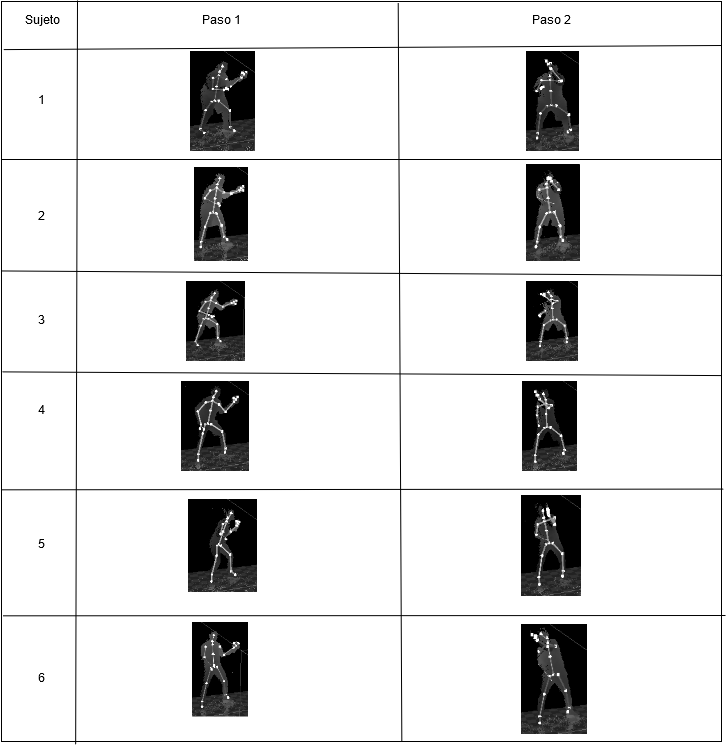
\includegraphics[width=445px,height=560px]{graphics/resultados/SETenisDeMesa.PNG} \\
	\textbf{Fuente:} Recuperado por los v\'ideos de trabajo de campo (ver instrumento \ref{ins:KinectStudio})
\end{figure}
\begin{figure}[H]
	\caption{Fotogramas de 7 sujetos del equipo de animaci\'on}
	\label{fig:fotogramaCheerleader}
	\centering
	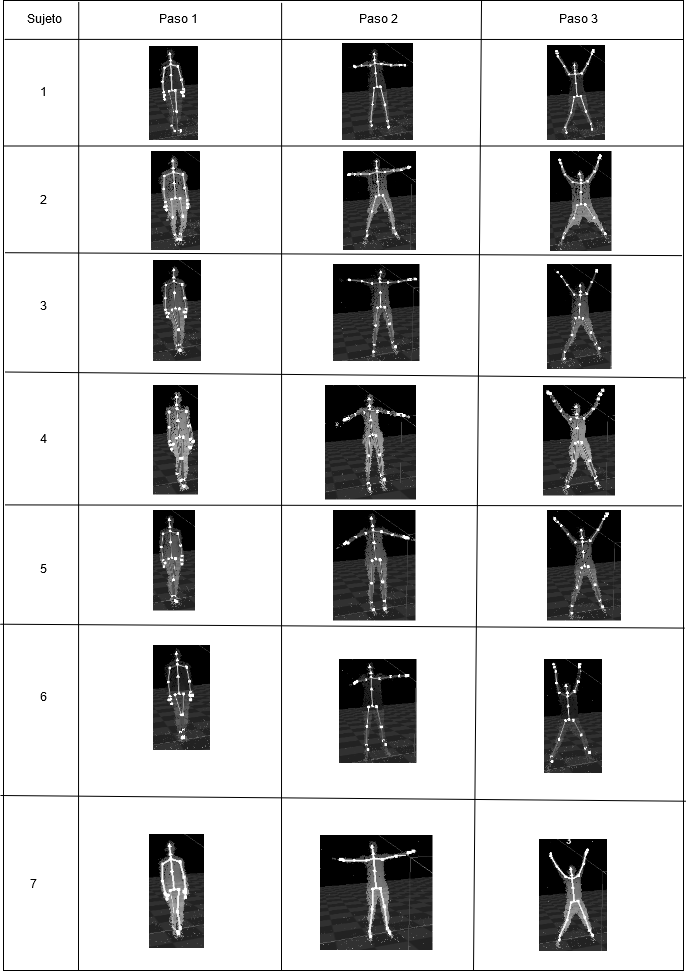
\includegraphics[width=445px,height=600px]{graphics/resultados/SECheerleaders.PNG} \\
	\textbf{Fuente:} Recuperado por los v\'ideos de trabajo de campo (ver instrumento \ref{ins:KinectStudio})
\end{figure}
\begin{figure}[H]
	\caption{Fotogramas de 7 sujetos del equipo de taekwondo}
	\label{fig:fotogramaTaekwondo}
	\centering
	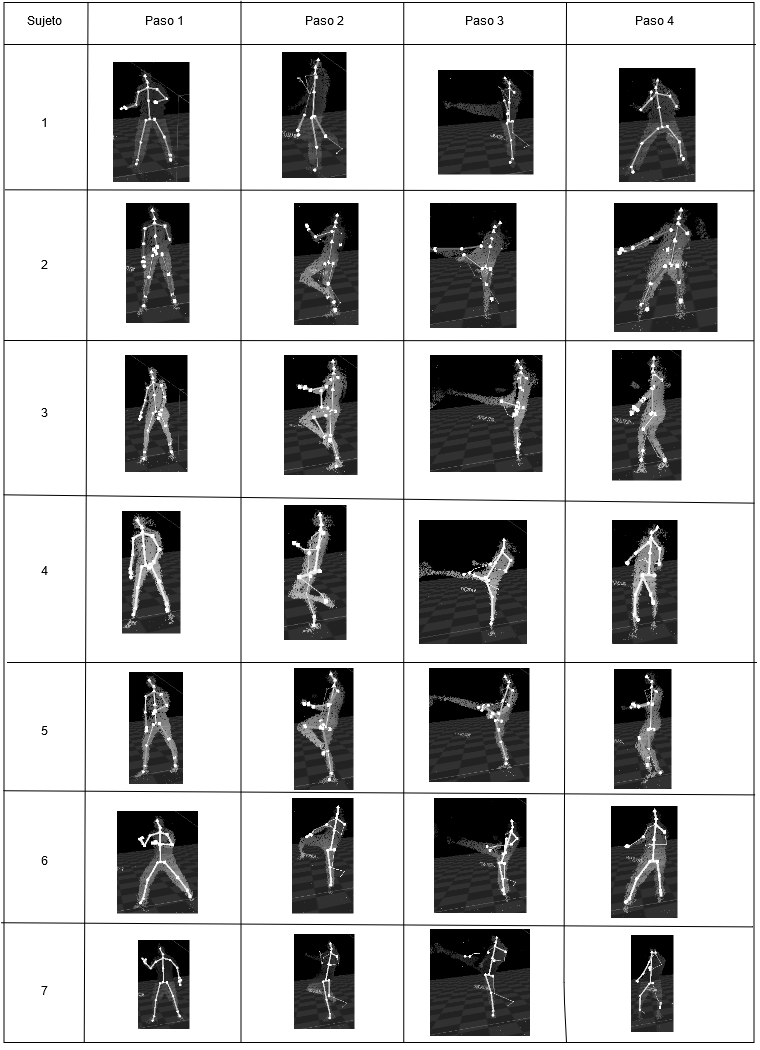
\includegraphics[width=445px,height=600px]{graphics/resultados/SETaekwondo.PNG} \\
	\textbf{Fuente:} Recuperado por los v\'ideos de trabajo de campo (ver instrumento \ref{ins:KinectStudio})
\end{figure}
\begin{landscape}
\section{Razones de fallo del seguimiento del esqueleto}
El seguimiento del esqueleto es un elemento  fundamental en cada fotograma, sin embargo se debe tomar en cuenta que puede fallar por varias razones, entre ellas se encuentran las siguientes fallas: del atleta (hombre), del sensor Kinect (m\'aquina), del lugar de trabajo (entorno y  medida), de la interacci\'on  con objetos o elementos externos (material) y de la preparaci\'on necesaria para realizar una rutina (m\'etodo):
\begin{figure}[H]
	\caption{Diagrama de ishikawa sobre el fallo del seguimiento del esqueleto}
	\label{fig:ishikawa}
	 \begin{center}
	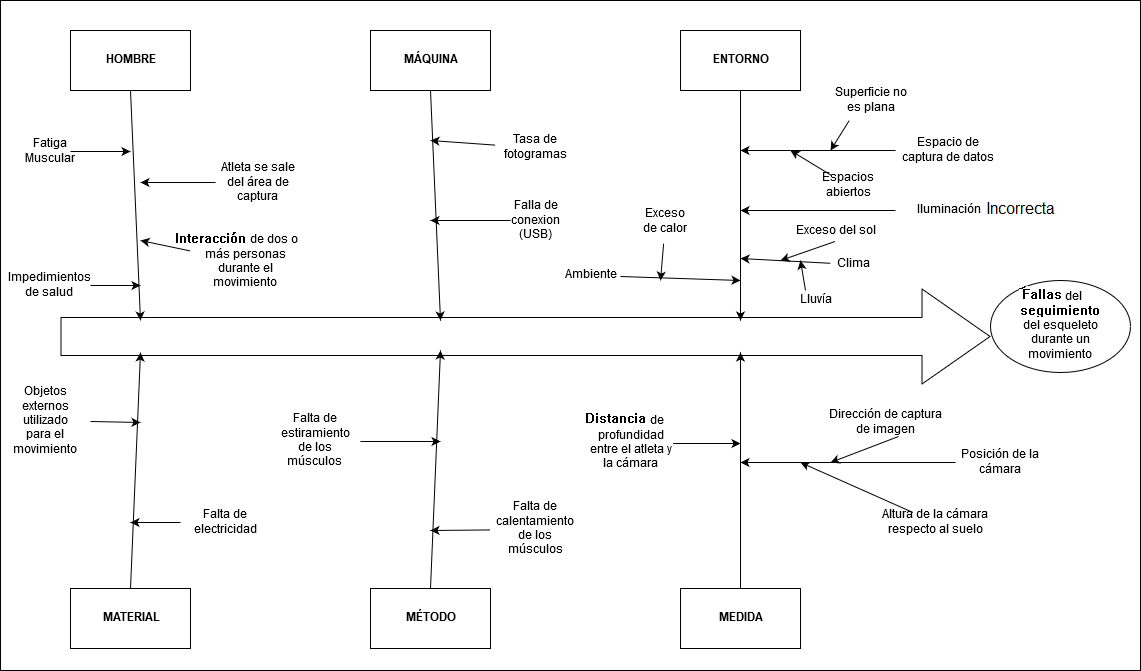
\includegraphics[width=500px,height=270px]{graphics/resultados/Ishi-SeguimientoDeEsqueleto.PNG}	 \\
	\end{center}
	\textbf{Fuente:} Este diagrama fue realizado con base a las observaciones del trabajo de campo, la cual el investigador observ\'o los sucesos en que fallaban el seguimiento del esqueleto, como por ejemplo las interrupciones de personas (generaba 2 o m\'as seguimientos de esqueletos) u objetos externos (interrupciones de pelotas de otros deportes), las fallas del hardware o software (falta de alimentaci\'on de energ\'ia), fallas en el ambiente que fue instalado el prototipo (exceso de calor, espacios cerrados, lluv\'ia, la iluminaci\'on incorrecta), fallas de la medici\'on (posici\'on del atleta o el sensor) y  fallas con respecto a la preparaci\'on del atleta (falta de calentamiento o impedimentos del salud del atleta, que conllevaba a realizar repeticiones no v\'alidas).
\end{figure}
\end{landscape}
\section{Proceso de etiquetaci\'on de un movimiento}
Consta de un conjunto de paneles de etiquetaciones de fotogramas, que se utilizaron para los entrenamientos y los testeos del algoritmo Random Forest Regression (reconocimiento de los pasos de un movimiento v\'alido), adem\'as por cada panel se debe tomar en cuenta los  siguientes elementos:
\begin{itemize}
\item Una l\'inea curvada (con forma de ese "S") que unifica 2 o m\'as puntos (representaci\'on de una repetici\'on que pasa por cada paso de un  movimiento v\'alido).
\item Espacios de color gris (momentos en que no se estan realizando un movimiento v\'alido).
\end{itemize}
As\'i mismo, estos resultados demuestran dos caracter\'isticas de la muestra de cada equipo deportivo:
\begin{itemize}
\item  La cantidad total de repeticiones de movimientos v\'alidos.
\item Cada atleta tiene distintas habilidades f\'isicas, debido que algunos realizaron m\'as repeticiones de lo solicitado (atletas que llevaban un tiempo en el equipo deportivo) y otros no (nuevos atletas del equipo deportivo).
\end{itemize}
\begin{table}[H]
	\caption{Etiquetaci\'on de fotogramas del equipo de tenis de mesa}
	\label{fig:etiquetaTenis}
	\centering
	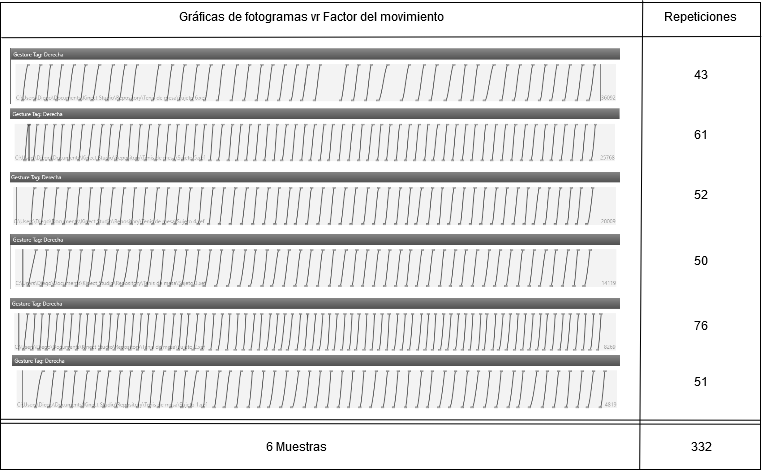
\includegraphics[width=445px,height=260px]{graphics/resultados/GraSegTenisDeMesa.PNG} \\
	\textbf{Fuente:} Recuperado por los v\'ideos etiquetados del trabajo de campo (ver instrumento \ref{ins:VisualGestureBuilder})
\end{table}
\begin{table}[H]
	\caption{Etiquetaci\'on de fotogramas del equipo de animaci\'on}
	\label{fig:etiquetaCheerleader}
	\centering
	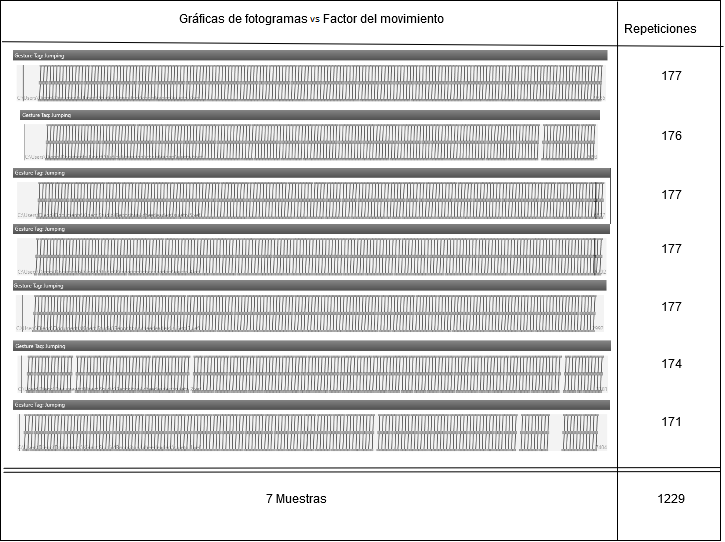
\includegraphics[width=445px,height=220px]{graphics/resultados/GraSegCheerleaders.PNG} \\
	\textbf{Fuente:} Recuperado por los v\'ideos etiquetados del trabajo de campo (ver instrumento \ref{ins:VisualGestureBuilder})
\end{table}
\begin{table}[H]
	\caption{Etiquetaci\'on de fotogramas del equipo de taekwondo}
	\label{fig:etiquetaTaekwondo}
	\centering
	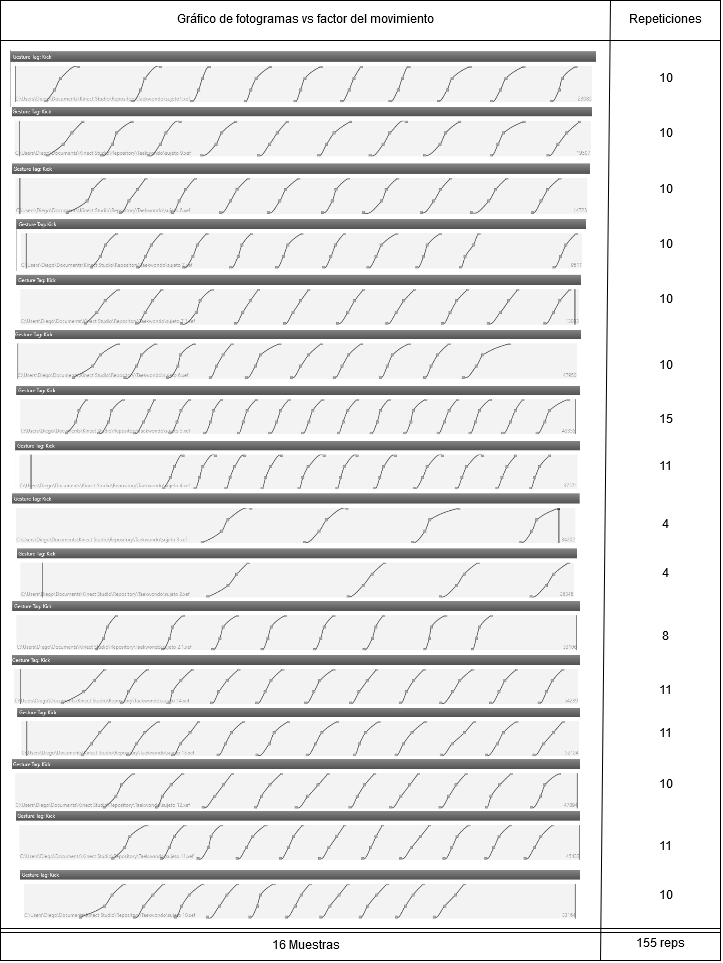
\includegraphics[width=445px,height=350px]{graphics/resultados/GraSegTaekwondo.PNG} \\
	\textbf{Fuente:} Recuperado por los v\'ideos etiquetados del trabajo de campo (ver instrumento \ref{ins:VisualGestureBuilder})
\end{table}
\section{Selecci\'on y pruebas del modelo} \label{res:chooseModel}
Por cada equipo deportivo se realiz\'o una tabla de informaci\'on del modelo de reconocimiento de los pasos de un movimiento v\'alido, la cual se divide en tres partes:
\begin{itemize}
\item  La primera parte se encontr\'o los errores de cada modelo y posteriormente se calcul\'o la media de cada error, la cual representa una \'idea de los  errores de todas las muestras de un equipo deportivo.
\item  La segunda parte se compone en la selecci\'on del submodelo que tenga la menor RECM, adem\'as de la aprobaci\'on o el rechazo de cada modelo,  as\'i mismo se encontr\'o el porcentaje de reconocimiento.
\item Finalmente, la tercera parte se muestra en caso que se apruebe el modelo, la cual detalla los intervalos de confianza para reconocer los pasos requeridos  de un movimiento.
\end{itemize}
\begin{table}[H]
\begin{center}
\caption{Modelos y pruebas del equipo de Taekwondo}
\label{tab:chooseTaekwondo}
\begin{tabular}{cccc}
\hline
\multicolumn{4}{|c|}{1. Datos de los errores de los submodelo} \\ \hline
\multicolumn{1}{|c|}{\textbf{Submodelo}} & \multicolumn{1}{c|}{\textbf{EMP}} & \multicolumn{1}{c|}{\textbf{DMA}} & \multicolumn{1}{c|}{\textbf{RECM}} \\ \hline
\multicolumn{1}{|c|}{1} & \multicolumn{1}{c|}{-0,03543} & \multicolumn{1}{c|}{0,301911} & \multicolumn{1}{c|}{+/-0,374544} \\ \hline
\multicolumn{1}{|c|}{2} & \multicolumn{1}{c|}{0,050888} & \multicolumn{1}{c|}{0,297433} & \multicolumn{1}{c|}{+/-0,393153} \\ \hline
\multicolumn{1}{|c|}{3} & \multicolumn{1}{c|}{0,200827} & \multicolumn{1}{c|}{0,214594} & \multicolumn{1}{c|}{+/-0,191583} \\ \hline
\multicolumn{1}{|c|}{\textbf{Promedio}} & \multicolumn{1}{c|}{0,072095} & \multicolumn{1}{c|}{0,271313} & \multicolumn{1}{c|}{+/-0,319760} \\ \hline
\multicolumn{1}{l}{} & \multicolumn{1}{l}{} & \multicolumn{1}{l}{} & \multicolumn{1}{l}{} \\ \hline
\multicolumn{4}{|c|}{2. Detalle del modelo} \\ \hline
\multicolumn{3}{|c|}{\textbf{Mejor submodelo}} & \multicolumn{1}{c|}{3} \\ \hline
\multicolumn{3}{|c|}{\textbf{Aprueba o rechaza el modelo}} & \multicolumn{1}{c|}{\begin{tabular}[c]{@{}c@{}}Rechaza\\ 0,31976  \textgreater{}=> 0.125\end{tabular}} \\ \hline
\multicolumn{3}{|c|}{\textbf{Recognition}} & \multicolumn{1}{c|}{-27.90\%} \\ \hline
\multicolumn{4}{l}{\textbf{Fuente:} C\'alculo de intervalos de confianza (ver f\'ormula \ref{frm:rangoConfiabilidad})}
\end{tabular}
\end{center}
\end{table}
\begin{table}[H]
\begin{center}
\caption{Modelos y pruebas del equipo de tenis de mesa }
\label{tab:chooseModelTenis}
\begin{tabular}{cccc}
\hline
\multicolumn{4}{|c|}{1. Datos de los errores de los submodelos} \\ \hline
\multicolumn{1}{|c|}{\textbf{Submodelo}} & \multicolumn{1}{c|}{\textbf{EMP}} & \multicolumn{1}{c|}{\textbf{DMA}} & \multicolumn{1}{c|}{\textbf{RECM}} \\ \hline
\multicolumn{1}{|c|}{1} & \multicolumn{1}{c|}{0,175144} & \multicolumn{1}{c|}{0,217553} & \multicolumn{1}{c|}{+/-0,236069} \\ \hline
\multicolumn{1}{|c|}{2} & \multicolumn{1}{c|}{0,022738} & \multicolumn{1}{c|}{0,113367} & \multicolumn{1}{c|}{+/-0,140393} \\ \hline
\multicolumn{1}{|c|}{3} & \multicolumn{1}{c|}{0,139513} & \multicolumn{1}{c|}{0,260699} & \multicolumn{1}{c|}{+/-0,342375} \\ \hline
\multicolumn{1}{|c|}{\textbf{Promedio}} & \multicolumn{1}{c|}{0,112465} & \multicolumn{1}{c|}{0,197206} & \multicolumn{1}{c|}{+/-0,239612} \\ \hline
\multicolumn{1}{l}{} & \multicolumn{1}{l}{} & \multicolumn{1}{l}{} & \multicolumn{1}{l}{} \\ \hline
\multicolumn{4}{|c|}{2. Detalle del modelo} \\ \hline
\multicolumn{3}{|c|}{\textbf{Mejor submodelo}} & \multicolumn{1}{c|}{2} \\ \hline
\multicolumn{3}{|c|}{\textbf{Aprueba o rechaza el modelo}} & \multicolumn{1}{c|}{\begin{tabular}[c]{@{}c@{}}Aprueba\\ 0,239612 \textless 0.25\end{tabular}} \\ \hline
\multicolumn{3}{|c|}{\textbf{Recognition}} & \multicolumn{1}{c|}{52.08\%} \\ \hline
\multicolumn{1}{l}{} & \multicolumn{1}{l}{} & \multicolumn{1}{l}{} & \multicolumn{1}{l}{} \\ \hline
\multicolumn{4}{|c|}{3. Detalle del paso del movimiento} \\ \hline
\multicolumn{2}{|c|}{\textbf{Detallle}} & \multicolumn{2}{c|}{\textbf{Intervalo de confianza}} \\ \hline
\multicolumn{1}{|c|}{Paso} & \multicolumn{1}{c|}{Etiqueta} & \multicolumn{1}{c|}{Inferior} & \multicolumn{1}{c|}{Superior} \\ \hline
\multicolumn{1}{|c|}{1} & \multicolumn{1}{c|}{0} & \multicolumn{1}{c|}{0} & \multicolumn{1}{c|}{0,239612} \\ \hline
\multicolumn{1}{|c|}{2} & \multicolumn{1}{c|}{1} & \multicolumn{1}{c|}{0,760388} & \multicolumn{1}{c|}{1} \\ \hline
\multicolumn{4}{l}{\textbf{Fuente:} C\'alculo de intervalos de confianza (ver f\'ormula \ref{frm:rangoConfiabilidad})}
\end{tabular}
\end{center}
\end{table}
\begin{table}[H]
\begin{center}
\caption{Modelos y pruebas del equipo de animaci\'on}
\label{tab:chooseCheerleader}
\begin{tabular}{cccc}
\hline
\multicolumn{4}{|c|}{1. Datos de los errores de los submodelos} \\ \hline
\multicolumn{1}{|c|}{\textbf{Submodelo}} & \multicolumn{1}{c|}{\textbf{EMP}} & \multicolumn{1}{c|}{\textbf{DMA}} & \multicolumn{1}{c|}{\textbf{RECM}} \\ \hline
\multicolumn{1}{|c|}{1} & \multicolumn{1}{c|}{0,02323} & \multicolumn{1}{c|}{0,038519} & \multicolumn{1}{c|}{+/-0,046957} \\ \hline
\multicolumn{1}{|c|}{2} & \multicolumn{1}{c|}{0,080008} & \multicolumn{1}{c|}{0,083864} & \multicolumn{1}{c|}{+/-0,076391} \\ \hline
\multicolumn{1}{|c|}{3} & \multicolumn{1}{c|}{0,032244} & \multicolumn{1}{c|}{0,04105} & \multicolumn{1}{c|}{+/-0,045347} \\ \hline
\multicolumn{1}{|c|}{\textbf{Promedio}} & \multicolumn{1}{c|}{+/-0,045161} & \multicolumn{1}{c|}{0,054478} & \multicolumn{1}{c|}{+/-0,056232} \\ \hline
\multicolumn{1}{l}{} & \multicolumn{1}{l}{} & \multicolumn{1}{l}{} & \multicolumn{1}{l}{} \\ \hline
\multicolumn{4}{|c|}{2. Detalle del modelo} \\ \hline
\multicolumn{3}{|c|}{\textbf{Mejor submodelo}} & \multicolumn{1}{c|}{3} \\ \hline
\multicolumn{3}{|c|}{\textbf{Aprueba o rechaza el modelo}} & \multicolumn{1}{c|}{\begin{tabular}[c]{@{}c@{}}Aprueba\\ 0,056232 \textless 0.165\end{tabular}} \\ \hline
\multicolumn{3}{|c|}{\textbf{Recognition}} & \multicolumn{1}{c|}{82.96\%} \\ \hline
\multicolumn{1}{l}{} & \multicolumn{1}{l}{} & \multicolumn{1}{l}{} & \multicolumn{1}{l}{} \\ \hline
\multicolumn{4}{|c|}{3. Detalle del paso del movimiento} \\ \hline
\multicolumn{2}{|c|}{\textbf{Detallle}} & \multicolumn{2}{c|}{\textbf{Intervalo de confianza}} \\ \hline
\multicolumn{1}{|c|}{Paso} & \multicolumn{1}{c|}{Etiqueta} & \multicolumn{1}{c|}{Inferior} & \multicolumn{1}{c|}{Superior} \\ \hline
\multicolumn{1}{|c|}{1} & \multicolumn{1}{c|}{0} & \multicolumn{1}{c|}{0} & \multicolumn{1}{c|}{0,056232} \\ \hline
\multicolumn{1}{|c|}{2} & \multicolumn{1}{c|}{0.5} & \multicolumn{1}{c|}{0,443768} & \multicolumn{1}{c|}{0,556232} \\ \hline
\multicolumn{1}{|c|}{3} & \multicolumn{1}{c|}{1} & \multicolumn{1}{c|}{0,943768} & \multicolumn{1}{c|}{1} \\ \hline
\multicolumn{4}{l}{\textbf{Fuente:} C\'alculo de intervalos de confianza (ver f\'ormula \ref{frm:rangoConfiabilidad})}
\end{tabular}
\end{center}
\end{table}
\section{Clasificaciones de movimiento v\'alidos e inv\'alidos} \label{res:clasiMov}
Estos resultados demuestran lo siguiente:
\begin{itemize}
\item  Cada submodelo fue entrenado con distintos datos de entrenamientos y testeos.
\item Por cada v\'ideo de entrenamiento de cada submodelo, se determin\'o  las repeticiones v\'alidas e inv\'alidas (de acuerdo a los intervalos de confianza  y el algoritmo clasificador de repetici\'on de un movimiento v\'alido).
\item A partir de las repeticiones inv\'alidas se pueden calcular el n\'umero de repeticiones inv\'alidas por no detectar el paso correspondiente (Es un par\'ametro que le puede ayudar al atleta a saber en cu\'al paso ha fallado los atletas de testeos). 
\end{itemize}
\begin{table}[H]
\begin{center}
\caption{C\'alculo de movimientos v\'alidos e inv\'alidos del equipo de animaci\'on}
\label{tab:validAnimacion}
\begin{tabular}{|c|c|c|c|c|c|c|c|}
\hline
\textbf{Detalles}    & \multicolumn{2}{c|}{\textbf{\begin{tabular}[c]{@{}c@{}}Las 1229 repeticiones\\  del movimiento\end{tabular}}}                          & \multicolumn{2}{c|}{\textbf{\begin{tabular}[c]{@{}c@{}}Las repeticiones \\ de testeos\end{tabular}}}                                      & \multicolumn{3}{c|}{\textbf{\begin{tabular}[c]{@{}c@{}}Las repeticiones no son \\ detectadas porque no se \\ detect\'o el paso No.\end{tabular}}} \\ \hline
\textbf{Submodelos}  & \textbf{\begin{tabular}[c]{@{}c@{}}De \\ entrenamientos\end{tabular}} & \textbf{\begin{tabular}[c]{@{}c@{}}De \\ testeos\end{tabular}} & \textbf{\begin{tabular}[c]{@{}c@{}}Son\\ v\'alidas\end{tabular}} & \textbf{\begin{tabular}[c]{@{}c@{}}Son \\ inv\'alidas\end{tabular}} & \textbf{1}                                     & \textbf{2}                                     & \textbf{3}                                    \\ \hline
1                    & 1053                                                                  & 176                                                            & 97                                                                & 79                                                                    & 2                                              & 25                                             & 52                                             \\ \hline
2                    & 1058                                                                  & 171                                                            & 50                                                                & 121                                                                   & 0                                              & 8                                              & 113                                            \\ \hline
3                    & 1055                                                                  & 174                                                            & 115                                                               & 59                                                                    & 0                                              & 43                                             & 16                                           \\ \hline
\textbf{Promedio}    & 1055                                                                  & 174                                                            & 88                                                                & 86                                                                    & 0                                              & 25                                             & 61                                            \\ \hline
\textbf{Porcentajes} & 85,84\%                                                               & 14,16\%                                                        & 50,57\%                                                           & 49,43\%                                                               & 0,00\%                                         & 29,07\%                                        & 70.93\%                                            \\ \hline
\multicolumn{8}{l}{\textbf{Fuente:} C\'alculo de porcentaje v\'alidos e inv\'alidos (ver F\'ormula \ref{frm:porcentajeClasificador})}
\end{tabular}
\end{center}
\end{table}
\section{Muestras de regresiones de los movimientos} \label{res:regretions}
Estos resultados muestran un ejemplo de las posibles regresiones que pueden implementar el modelo de m\'aquina de aprendizaje -i.e. Bosques de regresiones aleatorios-, adem\'as de comprobar que los modelos aceptados fueron entrenados con distintos datos de entrenamientos (uniformidad con los tiempos de capturas y una dispersi\'on con los recorridos de una articulaci\'on, durante la ejecuci\'on del  movimiento).
\begin{figure}[H]
	\caption{Regresi\'on distancia versus tiempo, del equipo animaci\'on}
	\label{fig:regrCheerleader}
	\centering
	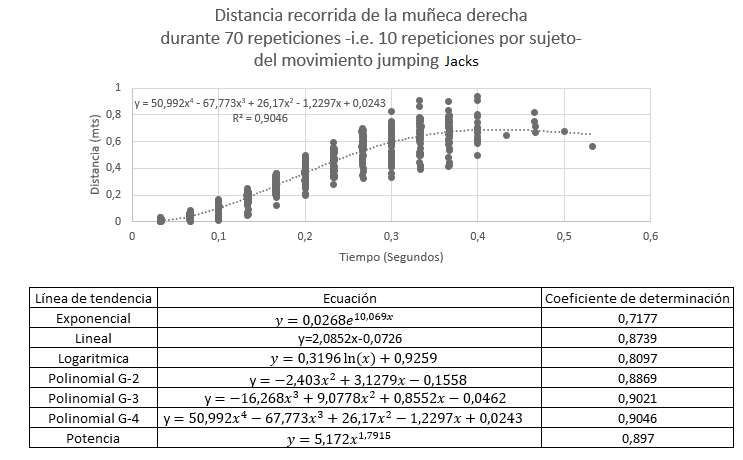
\includegraphics[width=445px,height=200px]{graphics/resultados/cluster-cheerleaders.PNG} \\
	\textbf{Fuente:} Recuperado por los v\'ideos etiquetados del trabajo de campo.
\end{figure}
\begin{figure}[H]
	\caption{Regresi\'on distancia versus tiempo  del equipo de tenis de mesa}
	\label{fig:regrTennisDeMesa}
	\centering
	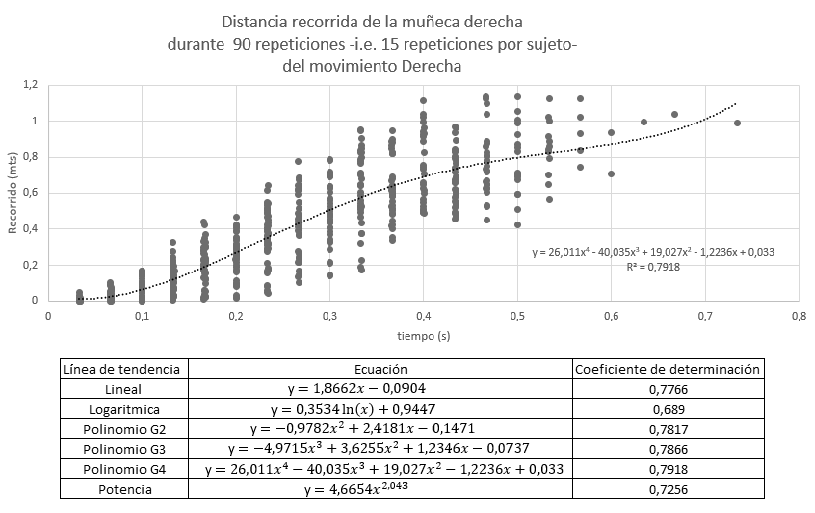
\includegraphics[width=445px,height=200px]{graphics/resultados/cluster-tennis.PNG} \\
	\textbf{Fuente:} Recuperado por los v\'ideos etiquetados del trabajo de campo.
\end{figure}
\section{Reconocimiento de movimiento}
En esta secci\'on se ense\~na los resultados de la interfaz gr\'afica del reconocimiento de repeticiones de un movimiento, la cual est\'a conformado por un conjunto de im\'agenes que muestran el seguimiento del esqueleto durante la ejecuci\'on de una repetici\'on, as\'i mismo en cada imagen se muestra los siguientes detalles:
\begin{itemize}
\item \textbf{Estado:} Tiene el valor de trabajo, debido que fue capturado durante el tiempo de trabajo en una rutina de tabata.
\item \textbf{Temporizador:} Tiempo de cuenta regresiva, la cual indica cu\'antos segundos le quedan al atleta en el estado de trabajo.
\item \textbf{Serie:} Le indica al atleta, cu\'al n\'umero de serie se est\'a ejecutando (Los resultados fueron capturado durante la serie No. 1 de trabajo).
\item \textbf{Repeticiones:} Le muestra al atleta la cantidad de repeticiones que lleva durante una   serie de trabajo (Se debe observar que este indicador incrementa en el \'ultimo paso de cada movimiento).
\item \textbf{Paso:} N\'umero que indica el \'ultimo paso ejecutado (Comenzando desde el valor 0). Se debe tomar en cuenta que dicho valor cambia dependiendo del factor de movimiento -i.e. Progreso-, es decir, se  reconoce cada paso del movimiento, ya que el valor del progreso se encuentra dentro de alg\'un intervalo de confianza (Ver las tablas de resultados de selecci\'on y pruebas del modelo).
\item \textbf{Progreso:} Factor del movimiento en tiempo real (obtenido a partir de la base de datos de gesturas), la cual va incrementado por cada paso que avance el atleta.
\item \textbf{Tiempo total:} Tiempo total que lleva actualmente el atleta (en los resultados se pueden ver que el atleta emplea una repetici\'on en un per\'iodo de d\'ecimas de segundos).
\end{itemize}
\begin{figure}[H]
	\caption{Reconocimiento del movimiento derecha}
	\label{fig:recognitionTenis}
	\centering
	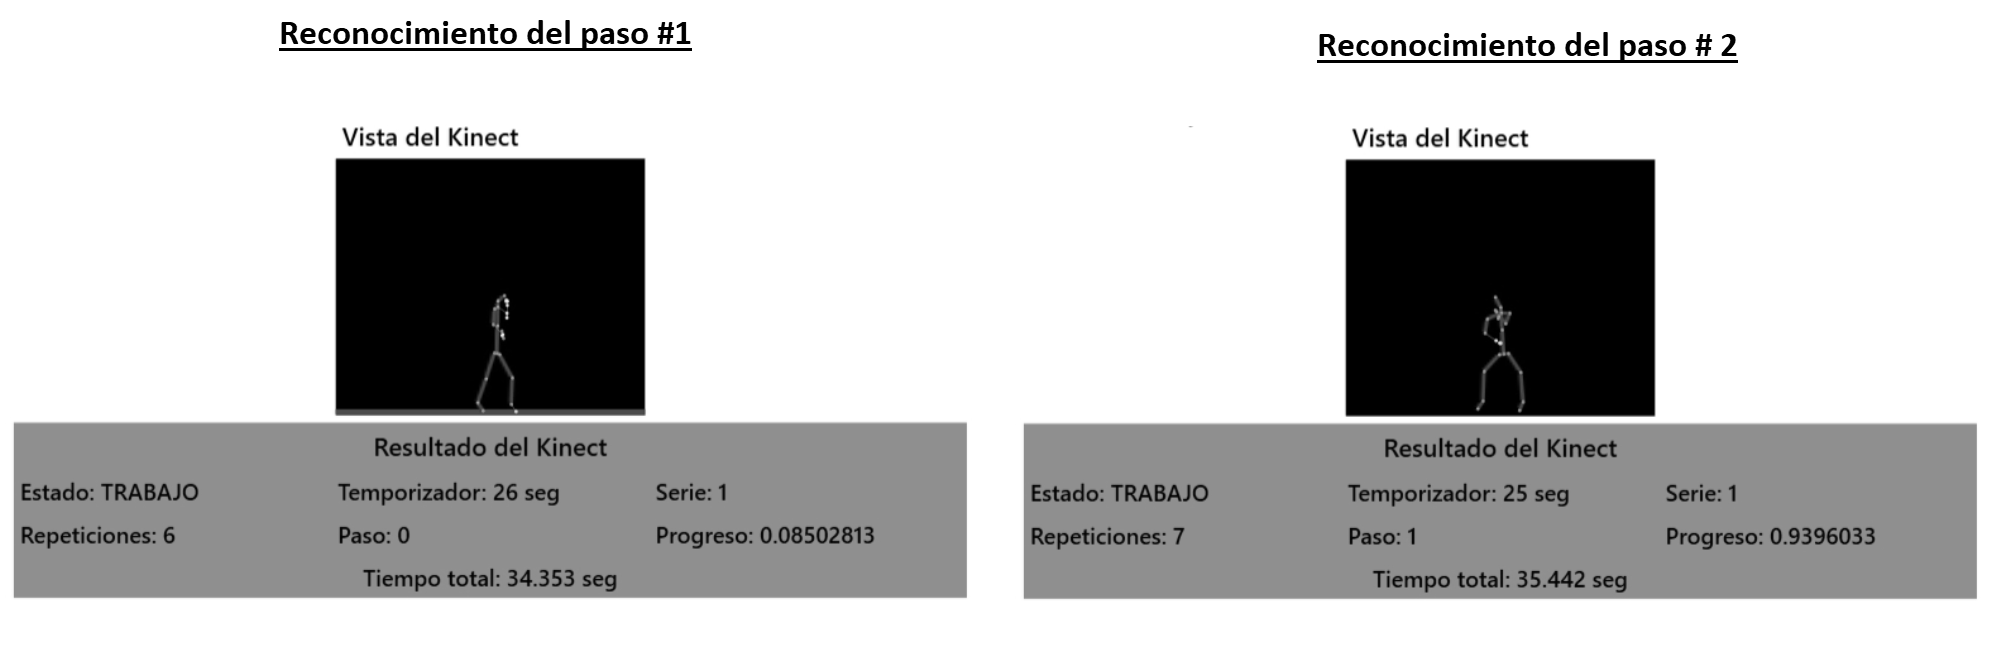
\includegraphics[width=420px,height=250px]{graphics/resultados/recognitionTennis.png} \\
	\textbf{Fuente:} sujeto de validaci\'on del modelo en tiempo real.
\end{figure}
\begin{figure}[H]
	\caption{Reconocimiento del movimiento jumping jacks}
	\label{fig:recognitionCheerleader}
	\centering
	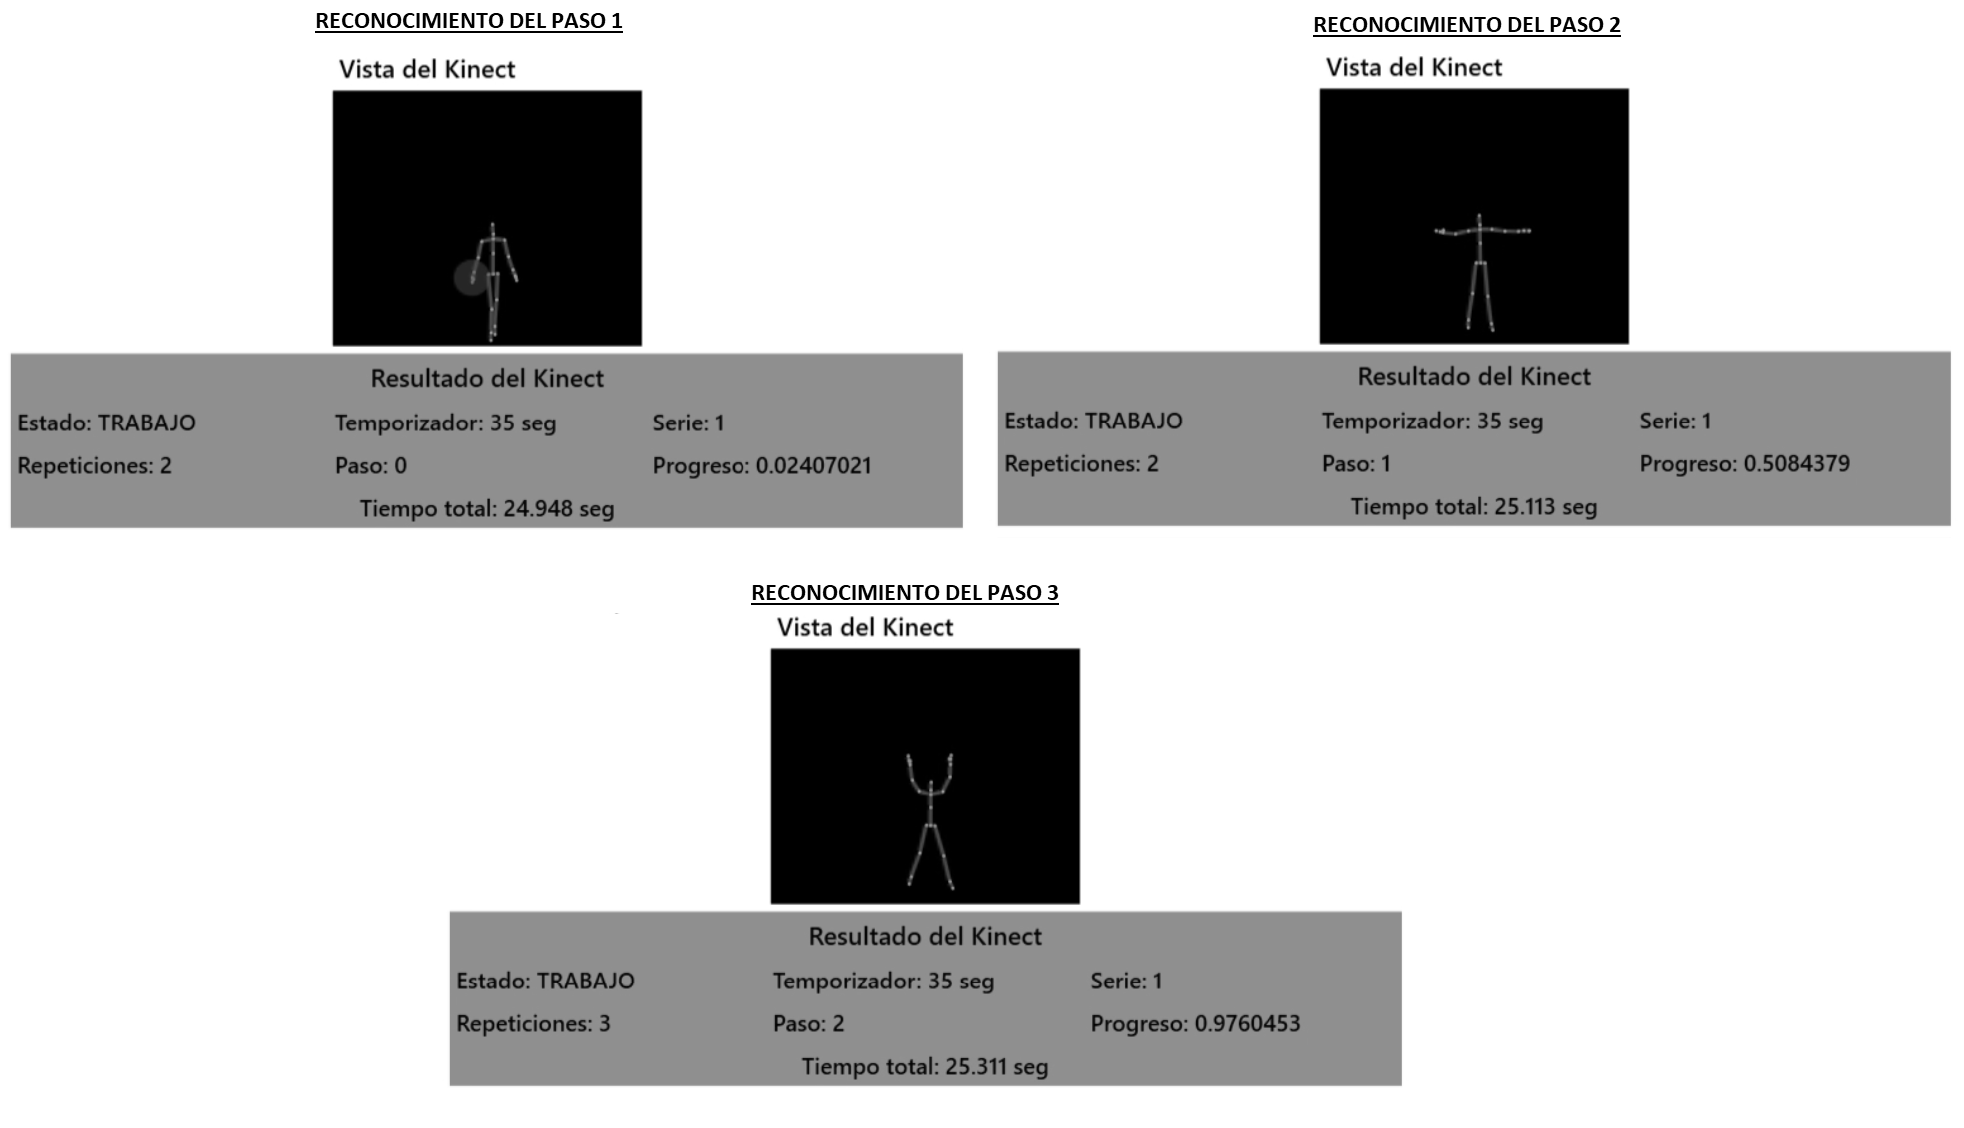
\includegraphics[width=430px,height=320px]{graphics/resultados/recognitionCheerleader.png} \\
	\textbf{Fuente:} sujeto de validaci\'on del modelo en tiempo real.
\end{figure}
\section{Validaci\'on del movimiento} \label{res:valResults}
A continuaci\'on se presenta la interfaz gr\'afica de los resultados de la rutina tabata por equipo deportivo, se debe considerar que para estos resultados se utilizaron atletas que no participaron en la toma de datos iniciales -i.e. Construcci\'on y testeo del modelo-, adem\'as de interpretar en dos partes los elementos del archivo de resultados de una rutina tabata (Ver anexos, c\'odigo \ref{code:tabata}):
\begin{itemize}
\item La primera parte consta de un conjunto de gr\'aficas que muestra de manera visual, el esfuerzo  de cada atleta durante la rutina tabata.
\item La segunda parte es un cuadro que detalla el  resumen ejecutivo de los resultados de la rutina tabata.
\end{itemize}
\begin{landscape}
\begin{chart}[H]
	\caption{Resultados del tabata del equipo de tenis de mesa}
	\label{fig:resTabTennis}
	\centering
	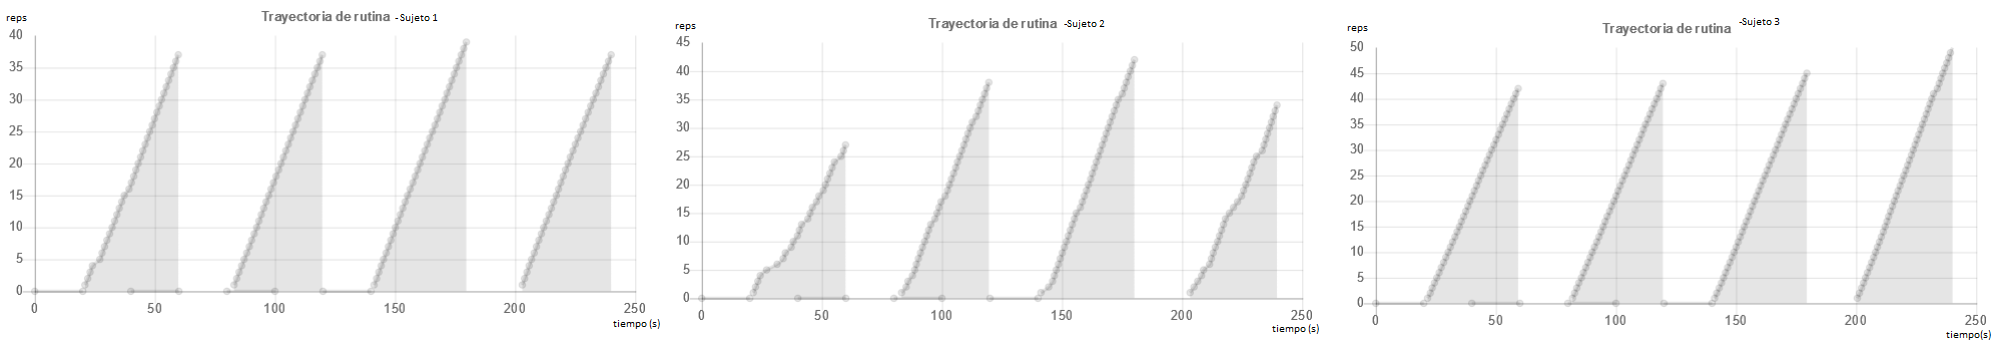
\includegraphics[width=610px,height=200px]{graphics/resultados/ResultRecognitionTenis.png} \\
	\textbf{Fuente:} Realizado con base a las observaciones del proceso de validaci\'on.
\end{chart}
\begin{table}[H]
\begin{center}
\caption{Detalle de la rutina tabata del equipo de tenis de mesa}
\label{tab:detailResultsTennis}
\begin{tabular}{|l|l|l|l|l|l|l|l|l|l|}
\hline
\textbf{Series} & \textbf{\begin{tabular}[c]{@{}l@{}}Trabajo\\ (segs)\end{tabular}} & \textbf{\begin{tabular}[c]{@{}l@{}}Descanso\\ (segs)\end{tabular}} & \textbf{\begin{tabular}[c]{@{}l@{}}Duraci\'on\\ (segs)\end{tabular}} & \textbf{Sujeto} & \textbf{\begin{tabular}[c]{@{}l@{}}Volumen de\\ repeticiones\end{tabular}} & \textbf{\begin{tabular}[c]{@{}l@{}}Repeticiones\\ m\'aximas en una\\ serie\end{tabular}} & \textbf{\begin{tabular}[c]{@{}l@{}}Tiempo m\'inimo\\ en una serie\\ (segs)\end{tabular}} & \textbf{\begin{tabular}[c]{@{}l@{}}Repeticiones \\ promedio por\\ serie\end{tabular}} & \textbf{\begin{tabular}[c]{@{}l@{}}Tiempo \\ promedio por\\ repetici\'on (segs)\end{tabular}} \\ \hline
\multirow{3}{*}{4} & \multirow{3}{*}{40} & \multirow{3}{*}{20} & \multirow{3}{*}{240} & 1 & 150 & 39 & 38.5440 & 38 & 0.7106 \\ \cline{5-10} 
 &  &  &  & 2 & 141 & 42 & 39.1050 & 35 & 0.7869 \\ \cline{5-10} 
 &  &  &  & 3 & 180 & 50 & 39.7980 & 45 & 0.3599 \\ \hline
 \multicolumn{10}{l}{\textbf{Fuente:} Gr\'afica de resultados del tabata del equipo de tenis de mesa}
\end{tabular}
\end{center}
\end{table}
\begin{chart}[H]
	\caption{Resultados del tabata del equipo de animaci\'on}
	\label{fig:resTabCheerleader}
	\centering
	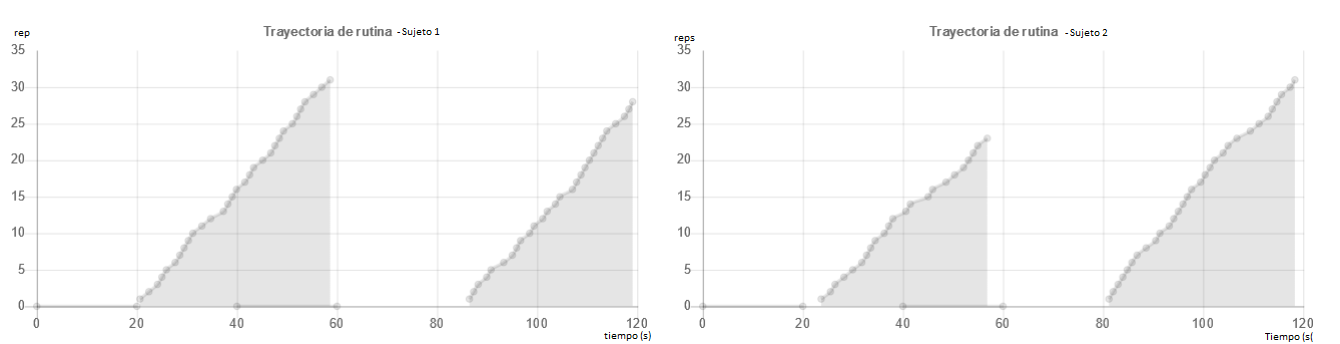
\includegraphics[width=610px,height=200px]{graphics/resultados/ResultRecognitionCheerleader.png} \\
	\textbf{Fuente:} Realizado con base a las observaciones del proceso de validaci\'on.
\end{chart}
\begin{table}[H]
\begin{center}
\caption{Detalle de la rutina tabata del equipo de animaci\'on}
\label{tab:detailResultsCheerleader}
\begin{tabular}{|l|l|l|l|l|l|l|l|l|l|}
\hline
\textbf{Series} & \textbf{\begin{tabular}[c]{@{}l@{}}Trabajo\\ (segs)\end{tabular}} & \textbf{\begin{tabular}[c]{@{}l@{}}Descanso\\ (segs)\end{tabular}} & \textbf{\begin{tabular}[c]{@{}l@{}}Duraci\'on\\ (segs)\end{tabular}} & \textbf{Sujeto} & \textbf{\begin{tabular}[c]{@{}l@{}}Volumen de\\ repeticiones\end{tabular}} & \textbf{\begin{tabular}[c]{@{}l@{}}Repeticiones\\ m\'aximas en una\\ serie\end{tabular}} & \textbf{\begin{tabular}[c]{@{}l@{}}Tiempo m\'inimo\\ en una serie\\ (segs)\end{tabular}} & \textbf{\begin{tabular}[c]{@{}l@{}}Repeticiones \\ promedio por\\ serie\end{tabular}} & \textbf{\begin{tabular}[c]{@{}l@{}}Tiempo \\ promedio por\\ repetici\'on (segs)\end{tabular}} \\ \hline
\multirow{2}{*}{2} & \multirow{2}{*}{40} & \multirow{2}{*}{20} & \multirow{2}{*}{120} & 1 & 59 & 31 & 38.3130 & 30 & 0.8284 \\ \cline{5-10} 
 &  &  &  & 2 & 54 & 31 & 37.5210 & 27 & 0.9301 \\ \hline
 \multicolumn{10}{l}{\textbf{Fuente} Gr\'afica de resultados del tabata del equipo de animaci\'on}
\end{tabular}
\end{center}
\end{table}
\end{landscape}